\section{有理函数}\label{sec:rational-maps-between-varieties}

为在下一节定义拟射影簇的维数作准备, 本节引入有理函数. 在仿射簇的情形, $X$ 上的有理函数定义为 $\operatorname{Frac}(K[X])$ 的元素, 即 $X$ 上多项式函数的商. 当 $X\subseteq\mathbb{P}^{n}$ 为拟射影簇时, 仍然考虑多项式的商, 但新的关键之处在于: 同次数的两个齐次多项式 $f,g\in K[x_{0},\ldots,x_{n}]$ 的商, 现在可以看作在开集 $X\setminus\mathcal{V}(g)$ 上定义一个正则函数. 基于这个观察, 我们用开集上的正则函数定义拟射影簇上的有理函数.

\begin{Definition}{拟射影簇上的有理函数}\leavevmode\label{def:rational-function-on-quasiprojective-variety}
设 $X$ 为拟射影簇. $X$ 上的一个\emph{有理函数}是数对 $(U,F)$ 的一个等价类, 其中 $U\subseteq X$ 为 $X$ 的稠密开子集, $F$ 为 $U$ 上的正则函数, 等价关系为
\[
  (U,F)\sim(V,G)\iff F(a)=G(a)\quad\forall a\in U\cap V.
\]
\end{Definition}

直观地说, $X$ 上的有理函数是\textquotedbl{}几乎处处\textquotedbl{}有定义的正则函数. 这与 $1/x$ 这样的商是 $\mathbb{A}^{1}\setminus\{0\}$ 上的正则函数大致相同, 而这个集合是 $\mathbb{A}^{1}$ 的\textquotedbl{}几乎全部\textquotedbl{}. 应当核对 Definition~\ref{def:rational-function-on-quasiprojective-variety} 中的关系是不是等价关系 (Exercise~\ref{ex:dense-open-rational-function-equivalence-relation}). 这里的关键是定义域稠密, 而不仅是开, 从而一个有理函数的两个代表的定义域必相交于稠密开子集. 引入等价关系的动机很简单: 一个有理函数的不同代表可能有不同的定义域, 但如果它们\textquotedbl{}几乎处处\textquotedbl{}相等, 我们就想把它们视为等价. 下面的例子说明这一等价概念.

\begin{Example}{$\mathbb{P}^{1}$ 上的有理函数}\leavevmode\label{ex:equivalent-rational-functions-on-projective-line}
令 $U=\mathbb{P}^{1}\setminus\{[1:0]\}$, $V=\mathbb{P}^{1}\setminus\{[1:0],[0:1]\}$, 考察由下式定义的正则函数 $F\in K[U]$ 和 $G\in K[V]$:
\[
  F([a:b])=\frac{a}{b}\qquad\text{和}\qquad G([a:b])=\frac{a^{2}}{ba}.
\]
注意 $U,V$ 都是 $\mathbb{P}^{1}$ 的稠密开子集, 因而 $(U,F)$ 和 $(V,G)$ 都给出 $\mathbb{P}^{1}$ 上的有理函数. 再者, 由于 $F$ 和 $G$ 在 $U\cap V$ 上相等, 可知 $(U,F)\sim(V,G)$. 直观地说, $F$ 和 $G$ 定义同一个有理函数, 只是因为定义 $G$ 的商约分后就是定义 $F$ 的商.
\end{Example}

$X$ 上的有理函数一般记为 $F:X\mathrel{\rightdasharrow} K$, 其中虚线箭头表示 $F$ 可能未在整个 $X$ 上定义. 有理函数 $F:X\mathrel{\rightdasharrow} K$ 的\emph{定义域}是它的所有代表的定义域的并. 由于稠密开子集对并封闭, 有理函数的定义域是 $X$ 的稠密开子集. 再者, 由正则函数的局部性质, 有理函数 $F:X\mathrel{\rightdasharrow} K$ 在其定义域上正则. 因此可以把有理函数的定义域看成它正则的最大集合.

和正则函数的集合一样, 有理函数的集合自然构成一个 $K$-代数 (Exercise~\ref{ex:rational-functions-form-algebra}), 从而得到以下定义.

\begin{Definition}{有理函数环}\leavevmode\label{def:ring-of-rational-functions}
令 $X$ 为拟射影簇. $X$ 上的\emph{有理函数环}记为 $K(X)$, 是所有有理函数 $F:X\mathrel{\rightdasharrow} K$ 构成的 $K$-代数.
\end{Definition}

由于拟射影簇的同构把开集及其上的正则函数环一一对应起来 (Corollary~\ref{cor:characterize-quasiprojective-isomorphisms-by-local-rings-of-functions}), 可知拟射影簇上的正则函数环是内在的 (Exercise~\ref{ex:rational-function-rings-invariant-under-isomorphism}).

下面看几个正则函数环的具体例子.

\begin{Example}{$K(\mathbb{P}^{n})=K(x_{1},\ldots,x_{n})$}\leavevmode\label{ex:rational-function-field-of-projective-space}
首先论证 $\mathbb{P}^{n}$ 上的有理函数都可用 $K[x_{0},\ldots,x_{n}]$ 中同次数的齐次多项式的商表示. 这样的商显然定义了 $\mathbb{P}^{n}$ 上的有理函数: 给定同次数的齐次多项式 $f,g\in K[x_{0},\ldots,x_{n}]$, $f/g$ 在开集 $U=\mathbb{P}^{n}\setminus\mathcal{V}(g)$ 上定义一个正则函数, 该开集稠密, 因为 $\mathbb{P}^{n}$ 不可约. 反过来, 给定 $\mathbb{P}^{n}$ 上由开子集 $U\subseteq\mathbb{P}^{n}$ 上的正则函数 $F:U\to K$ 表示的任一有理函数, Lemma~\ref{lem:regular-functions-on-projective-open-subsets-are-global-quotients} 表明, 存在同次数的齐次多项式 $f,g\in K[x_{0},\ldots,x_{n}]$, 使 $\mathcal{V}(g)\cap U=\varnothing$, 且在 $U$ 上有 $F=f/g$. 由此得
\[
  (U,F)\sim(\mathbb{P}^{n}\setminus\mathcal{V}(g),f/g),
\]
这说明 $\mathbb{P}^{n}$ 上的任意有理函数都能表示为同次数的齐次多项式的商, 如所断言.

稍加思考可知, 两个商 $f_{1}/g_{1}$ 和 $f_{2}/g_{2}$ 定义同一个 $\mathbb{P}^{n}$ 上的有理函数, 当且仅当 $f_{1}g_{2}-f_{2}g_{1}=0$. 这与定义 $K(x_{0},\ldots,x_{n})=\operatorname{Frac}(K[x_{0},\ldots,x_{n}])$ 中元素的关系相同. 换句话说, 可以把 $K(\mathbb{P}^{n})$ 与 $K(x_{0},\ldots,x_{n})$ 的一个子环等同, 该子环由分子与分母都是同次数齐次多项式的商组成. 关于 $x_{0}$ 去齐次化后, 得到 $K(\mathbb{P}^{n})=K(x_{1},\ldots,x_{n})$.
\end{Example}

\begin{Example}{$\mathcal{V}(xy)\subseteq\mathbb{P}^{2}$ 上的有理函数}\leavevmode\label{ex:rational-functions-on-union-of-projective-lines}
令 $X$ 为可约簇 $\mathcal{V}(xy)\subseteq\mathbb{P}^{2}$, 由两个分支 $\mathcal{V}(x)$ 和 $\mathcal{V}(y)$ 组成. 定义有理函数 $F:X\mathrel{\rightdasharrow} K$ 和 $G:X\mathrel{\rightdasharrow} K$ 为
\[
  F([a:b:c])=a/c\qquad\text{和}\qquad G([a:b:c])=b/c,
\]
它们都定义在稠密开集 $U=X\setminus\{[1:0:0],[0:1:0]\}$ 上. 因为 $F,G$ 都不在其定义域上消没, 它们在 $K(X)$ 中都不为零. 但乘积 $F\cdot G$ 在 $U$ 上消没. 由此可见, $X$ 上的有理函数环不是整环, 特别地, 它不是域.
\end{Example}

在前面的例子中, 我们观察到, 不可约簇 $\mathbb{P}^{n}$ 上的有理函数环不仅是环, 还是域; 而可约簇 $\mathcal{V}(xy)\subseteq\mathbb{P}^{2}$ 上的有理函数环不是域, 因为它有零因子. 下一个结果自然推广这些观察.

\begin{Proposition}{不可约簇上的有理函数}\leavevmode\label{prop:rational-function-ring-is-field-iff-irreducible}
设 $X$ 为拟射影簇. 则 $K(X)$ 是域, 当且仅当 $X$ 不可约.
\end{Proposition}
\begin{Proof}
Exercise~\ref{ex:prove-rational-function-ring-is-field-criterion}.
\end{Proof}

作为 Proposition~\ref{prop:rational-function-ring-is-field-iff-irreducible} 的结果, 当 $X$ 是不可约拟射影簇时, 通常把 $K(X)$ 称为\emph{有理函数域}.

和对正则函数所做的一样, 也应解决仿射情形下记号 $K(X)$ 的双重用法. 为此, 需要确认当 $X$ 是不可约仿射簇时, 它的函数域 (定义为其坐标环的分式域) 与对应的拟射影簇上的有理函数域相同.

\begin{Proposition}{仿射簇上的有理函数域}\leavevmode\label{prop:affine-function-field-equals-rational-function-field}
设 $X_{0}\subseteq\mathbb{A}^{n}$ 为不可约闭集, $X=j_{0}(X_{0})\subseteq\mathbb{P}^{n}$ 为对应的拟射影簇. 则 $X$ 上的有理函数域与 $X_{0}$ 的函数域之间有典范 $K$-代数同构
\[
  K(X)=K(X_{0}).
\]
\end{Proposition}
\begin{Proof}
回顾 $K(X_{0})=\operatorname{Frac}(K[X_{0}])$. 因此 $K(X_{0})$ 的元素可表示为 $F_{0}/G_{0}$, 其中 $F_{0},G_{0}\in K[X_{0}]$ 且 $G_{0}\ne0$. 选取多项式代表 $f_{0},g_{0}\in K[x_{1},\ldots,x_{n}]$, 使 $F_{0}=[f_{0}]$, $G_{0}=[g_{0}]$. 令 $f,g\in K[x_{0},\ldots,x_{n}]$ 为同次数的齐次多项式, 关于 $x_{0}$ 去齐次化分别得到 $f_{0}$ 和 $g_{0}$. 由于 $f/g$ 在 $X\setminus\mathcal{V}(g)$ 上正则, 得到有理函数
\[
  f/g:X\mathrel{\rightdasharrow} K.
\]
先验证映射 $F_{0}/G_{0}\mapsto f/g$ 在 $K(X_{0})$ 上良定义. 若 $F'_{0}/G'_{0}$ 是等价的商, 则 $F_{0}G'_{0}=F'_{0}G_{0}\in K[X_{0}]$. 因此, 任意多项式代表 $F'_{0}=[f'_{0}]$ 和 $G'_{0}=[g'_{0}]$ 满足 $f_{0}g'_{0}-f'_{0}g_{0}\in\mathcal{I}(X_{0})$. 于是, 若 $f',g'$ 为关于 $x_{0}$ 去齐次化得到 $f'_{0},g'_{0}$ 的同次数齐次多项式, 则 $f/g$ 和 $f'/g'$ 在稠密开子集 $X\setminus\mathcal{V}(gg')\subseteq X$ 上相等, 所以它们表示 $X$ 上同一个有理函数. 因此, 上述构造给出良定义的映射 $\phi:K(X_{0})\to K(X)$:
\[
  \phi(F_{0}/G_{0})=f/g.
\]
容易看出 $\phi$ 是同态, 只需再核对 $\phi$ 是双射.

为证明 $\phi$ 为单射, 假设 $\phi(F_{0}/G_{0})=f/g=0\in K(X)$. 则 $f/g$ 必在 $X$ 的某个稠密开子集上消没, 从而 $f$ 在 $X$ 上消没. 这只有在 $F_{0}$ 在 $X_{0}$ 上消没时才可能, 所以 $F_{0}/G_{0}=0\in K(X_{0})$, 证得单射性.

为证明 $\phi$ 为满射, 令 $F:X\mathrel{\rightdasharrow} K$ 为有理函数. 给定 $F$ 的定义域中的任意一点 $p$, $F$ 在 $p$ 处正则, 因而存在齐次多项式 $f,g$, 使 $p\notin\mathcal{V}(g)$, 且 $F=f/g$ 在 $X\setminus\mathcal{V}(g)$ 上成立. 关于 $x_{0}$ 去齐次化后, 得到多项式 $f_{0},g_{0}\in K[x_{1},\ldots,x_{n}]$, 使 $\phi([f_{0}]/[g_{0}])=F$. 这证明了满射性, 从而完成证明.
\end{Proof}

Proposition~\ref{prop:affine-function-field-equals-rational-function-field} 表明, 不可约仿射簇上的有理函数域就是其坐标环的分式域. 实际上, 知道如何在这个很特殊的情形下计算 $K(X)$, 就能计算任何不可约拟射影簇 $X$ 的 $K(X)$. 这是下一个结果的推论.

\begin{Proposition}{$K(X)$ 由稠密开子簇确定}\leavevmode\label{prop:rational-functions-determined-on-dense-open-subvariety}
设 $X$ 为拟射影簇, $U\subseteq X$ 为 $X$ 的稠密开子簇. 则
\[
  K(X)=K(U).
\]
\end{Proposition}
\begin{Proof}
$U$ 的任一稠密开子集也是 $X$ 的稠密开子集. 因此, 定义在 $V\subseteq U$ 上的有理函数 $F:U\mathrel{\rightdasharrow} K$ 也给出定义在同一个集合 $V\subseteq X$ 上的有理函数 $F:X\mathrel{\rightdasharrow} K$. 这给出典范包含 $K(U)\subseteq K(X)$.

反过来, 若 $G:X\mathrel{\rightdasharrow} K$ 为定义在稠密开集 $W\subseteq X$ 上的有理函数, 则 $W\cap U$ 是 $X$ 的稠密开集, 且 $(U,G)\sim(U\cap W,G|_{U\cap W})$. 由于 $U\cap W$ 是 $U$ 的稠密开集, $G\in K(X)$ 等价于来自 $K(U)$ 的有理函数, 从而 $K(U)=K(X)$.
\end{Proof}

结合 Propositions~\ref{prop:affine-function-field-equals-rational-function-field} 和~\ref{prop:rational-functions-determined-on-dense-open-subvariety}, 再利用每个拟射影簇都是局部仿射的这一事实, 任意不可约拟射影簇上的有理函数域都可以归结为一个仿射簇的函数域来计算. 下面的例子说明这一策略.

\begin{Example}{再看 $K(\mathbb{P}^{n})=K(x_{1},\ldots,x_{n})$}\leavevmode\label{ex:projective-function-field-via-affine-patch}
考察仿射开片 $\mathbb{A}^{n}_{0}\subseteq\mathbb{P}^{n}$. 此时有
\[
  K(\mathbb{P}^{n})=K(\mathbb{A}^{n}_{0})
  =\operatorname{Frac}(K[x_{1},\ldots,x_{n}])=K(x_{1},\ldots,x_{n}),
\]
其中第一个等式由 Proposition~\ref{prop:rational-functions-determined-on-dense-open-subvariety} 得到, 第二个由 Proposition~\ref{prop:affine-function-field-equals-rational-function-field} 得到.
\end{Example}

\begin{Example}{$\mathcal{V}(wx^{2}-y^{3})$ 上的有理函数域}\leavevmode\label{ex:projective-cuspidal-cubic-function-field}
考察射影簇 $X=\mathcal{V}(wx^{2}-y^{3})\subseteq\mathbb{P}^{2}$, 它包含仿射开片 $X_{0}=\mathcal{V}_{\mathbb{A}}(x^{2}-y^{3})\subseteq\mathbb{A}^{2}$ 作为稠密开子集. 我们已在 Example~\ref{ex:function-field-of-cusp} 中计算 $K(X_{0})$, 得到
\[
  K(X)=K(X_{0})=\operatorname{Frac}\left(\frac{K[x,y]}{\langle x^{2}-y^{3}\rangle}\right)
  \cong K(t),
\]
\BookPairedFigure{
其中同构由将 $[x]$ 与 $t^{3}$ 等同, 并将 $[y]$ 与 $t^{2}$ 等同给出.

由于 $K(X)\cong K(\mathbb{P}^{1})$, 读者可能猜想 $X\cong\mathbb{P}^{1}$. 这个猜想是错的, 但一个较弱的结论成立. 虽然两个簇并非处处同构, 但从 $X$ 去掉尖点 $[1:0:0]$, 从 $\mathbb{P}^{1}$ 去掉它的原像 $[1\ 0]$ 后, 右图所示映射成为同构.
}{
\phantomsection\label{fig:projective-cuspidal-cubic-birational-map}%
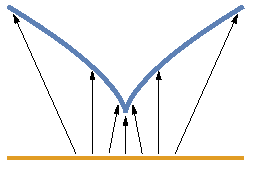
\includegraphics[width=\linewidth]{figures/projective-cuspidal-cubic-birational-map.pdf}
}
下面将在 Example~\ref{ex:projective-cuspidal-cubic-birational-to-line} 中回到这个讨论.
\end{Example}

\begin{Example}{$\mathcal{V}(w^{3}+x^{3}+y^{3})$ 上的有理函数域}\leavevmode\label{ex:irreducible-projective-cubic-not-isomorphic-to-line}
令 $X=\mathcal{V}(w^{3}+x^{3}+y^{3})\subseteq\mathbb{P}^{2}$. 与前一例类似, 可通过计算仿射部分 $X_{0}$ 的函数域来计算 $K(X)$, 得到
\[
  K(X)=K(X_{0})=\operatorname{Frac}\left(\frac{K[x,y]}{\langle1+x^{3}+y^{3}\rangle}\right).
\]
我们在 Example~\ref{ex:fermat-cubic-not-rational} 中证明, 对任意 $d$ 都有 $K(X_{0})\not\cong K(t_{1},\ldots,t_{d})$. 由于同构的簇有同构的有理函数环 (Exercise~\ref{ex:rational-function-rings-invariant-under-isomorphism}), 可知对任意 $d$ 有 $X\not\cong\mathbb{P}^{d}$. 特别地, $X\not\cong\mathbb{P}^{1}$. 这为第~\ref{sec:isomorphisms-of-projective-varieties}~节讨论的一种现象给出了具体例子: 不同于不可约二次曲线, $\mathbb{P}^{2}$ 中的不可约三次曲线不必同构于 $\mathbb{P}^{1}$.
\end{Example}

既然正则函数是正则映射的特例, 可能就会预期有理函数是更一般的有理映射的特例, 事实确实如此. 实际上, 有理映射的定义几乎逐字仿照有理函数的定义.

\begin{Definition}{有理映射}\leavevmode\label{def:rational-map-of-quasiprojective-varieties}
令 $X,Y$ 为拟射影簇. 从 $X$ 到 $Y$ 的一个\emph{有理映射}是数对 $(U,F)$ 的一个等价类, 其中 $U\subseteq X$ 是 $X$ 的稠密开子集, $F:U\to Y$ 是正则映射, 等价关系为
\[
  (U,F)\sim(V,G)\iff F(a)=G(a)\quad\forall a\in U\cap V.
\]
将有理映射记为 $F:X\mathrel{\rightdasharrow} Y$. 有理映射 $F:X\mathrel{\rightdasharrow} Y$ 的\emph{定义域}记为 $U_{F}\subseteq X$, 是 $F$ 的所有代表的定义域的并, 而 $F$ 的\emph{像}为 $F(U_{F})\subseteq Y$.
\end{Definition}

直观地说, 有理映射是拟射影簇之间\textquotedbl{}几乎处处\textquotedbl{}有定义的映射. 在研究有理映射时, 与\textquotedbl{}同构\textquotedbl{}相应的概念是双有理等价.

\begin{Definition}{双有理等价}\leavevmode\label{def:birational-equivalence}
令 $X,Y$ 为拟射影簇. \emph{双有理等价}是有理映射 $F:X\mathrel{\rightdasharrow} Y$, 使存在有理映射 $G:Y\mathrel{\rightdasharrow} X$, 其中 $G\circ F$ 是等价于 $\operatorname{id}_{X}$ 的有理映射, $F\circ G$ 是等价于 $\operatorname{id}_{Y}$ 的有理映射. 若 $X$ 与 $Y$ 之间存在双有理等价, 就称 $X$ 与 $Y$ \emph{双有理}.
\end{Definition}

注意, 复合 $G\circ F$ 定义在 $U_{F}$ 中映入 $U_{G}$ 的点所构成的开集上. 因此 Definition~\ref{def:birational-equivalence} 中要求 $G\circ F$ 是有理映射, 意味着这个集合必在 $X$ 中稠密. 实质上, 双有理的簇\textquotedbl{}几乎处处\textquotedbl{}同构, 给出严格弱于同构的关系. 下一例具体说明一个双有理等价: Example~\ref{ex:projective-cuspidal-cubic-function-field} 的带尖点曲线与射影直线双有理.

\begin{Example}{$\mathcal{V}(wx^{2}-y^{3})$ 与 $\mathbb{P}^{1}$ 双有理}\leavevmode\label{ex:projective-cuspidal-cubic-birational-to-line}
如 Example~\ref{ex:projective-cuspidal-cubic-function-field} 一样, 令 $X=\mathcal{V}(wx^{2}-y^{3})\subseteq\mathbb{P}^{2}$. 则 $X$ 与 $\mathbb{P}^{1}$ 双有理. 为了看出这一点, 考察由下式给出的正则映射 $F:\mathbb{P}^{1}\to X$:
\[
  F([a:b])=[a^{3}:b^{3}:ab^{2}].
\]
虽然 $F$ 没有逆映射, 但有一个有理映射 $G:X\mathrel{\rightdasharrow}\mathbb{P}^{1}$, 由
\[
  G([a:b:c])=[c:b]
\]
给出. 它定义在 $X$ 中 $x$ 和 $y$ 不同时为零的稠密开子集上, 并且作为有理映射与 $G$ 互逆. 从图像上看, 这就是说, 从 $X$ 去掉尖点 $[1:0:0]$ (见 Example~\ref{ex:projective-cuspidal-cubic-function-field}), 从 $\mathbb{P}^{1}$ 去掉它的原像 $[1:0]$ 后, 映射 $F$ 和 $G$ 成为同构.
\end{Example}

正如同构的拟射影簇具有同构的正则函数环, 双有理的拟射影簇具有同构的有理函数环. 例如, 对 Example~\ref{ex:projective-cuspidal-cubic-birational-to-line} 中的 $X$, Example~\ref{ex:projective-cuspidal-cubic-function-field} 的结果表明
\[
  K(X)\cong K(t)\cong K(\mathbb{P}^{1}),
\]
这反映了 Example~\ref{ex:projective-cuspidal-cubic-birational-to-line} 中的双有理等价. 事实上, 与正则函数的情形不同, 上述断言的逆命题也成立. 这里陈述这一结果, 但因为双有理等价在本书余下部分不居核心地位, 把证明留作习题.

\begin{Proposition}{双有理性与有理函数}\leavevmode\label{prop:birational-iff-rational-function-rings-isomorphic}
令 $X,Y$ 为拟射影簇. 则 $X$ 与 $Y$ 双有理, 当且仅当 $K(X)$ 与 $K(Y)$ 是同构的 $K$-代数.
\end{Proposition}
\begin{Proof}
Exercises~\ref{ex:pullback-of-rational-functions-under-dominant-map} 和~\ref{ex:construct-rational-map-from-function-ring-homomorphism}.
\end{Proof}

代数几何中有一个大而活跃的分支, 称为\emph{双有理几何}, 专门按簇之间是否双有理来对簇分类. 由于双有理的簇\textquotedbl{}几乎处处\textquotedbl{}同构, 它们具有某些共同属性: 由 Proposition~\ref{prop:birational-iff-rational-function-rings-isomorphic}, 它们的有理函数环相同, 所以 (如下一节将看到的) 它们的维数相同. 但双有理的簇也可能在关键方面不同. 例如, 一个可能是光滑的 (在下下节将遇到拟射影簇的这一概念), 而另一个可能是奇异的, Example~\ref{ex:projective-cuspidal-cubic-birational-to-line} 中的一对簇正是如此. 为一个给定奇异簇寻找与它双有理的光滑簇, 称为\emph{消解奇点}, 它建立在对奇点作爆破的概念之上, 是代数几何中的基本课题. 本章稍后会进一步略述这个概念.

\BookExerciseHeading
\begin{BookExercises}
  \item\label{ex:dense-open-rational-function-equivalence-relation}
  \begin{enumerate}
    \item 证明 Definition~\ref{def:rational-function-on-quasiprojective-variety} 中的关系是等价关系.
    \item 举例说明, 若不要求开集稠密, Definition~\ref{def:rational-function-on-quasiprojective-variety} 中的关系可能不具有传递性.
  \end{enumerate}
  \item\label{ex:rational-functions-form-algebra} 令 $X$ 为拟射影簇. 给定稠密开子集 $U,V\subseteq X$, 正则函数 $F:U\to K$ 和 $G:V\to K$, 以及标量 $\lambda\in K$, 用自然方式定义和, 积及标量倍数:
  \[
    F+G:U\cap V\to K,\qquad FG:U\cap V\to K,\qquad
    \text{以及 }\lambda F:U\to K.
  \]
  解释为何这些运算在有理函数的等价类上良定义, 并证明它们赋予有理函数的集合以 $K$-代数结构.
  \item\label{ex:rational-function-rings-invariant-under-isomorphism} 令 $X,Y$ 为同构的拟射影簇. 证明它们的有理函数环同构: $K(X)\cong K(Y)$.
  \item\label{ex:prove-rational-function-ring-is-field-criterion} 证明 Proposition~\ref{prop:rational-function-ring-is-field-iff-irreducible}.
  \item\label{ex:rational-function-ring-splits-over-irreducible-components} 令 $X$ 为拟射影簇, 不可约分支为 $X_{1},\ldots,X_{k}$. 证明
  \[
    K(X)=K(X_{1})\oplus\cdots\oplus K(X_{k}).
  \]
  \item\label{ex:affine-space-birational-to-projective-space} 证明 $\mathbb{A}^{n}$ 与 $\mathbb{P}^{n}$ 双有理.
  \item\label{ex:birational-equivalence-iff-dense-open-isomorphism} 令 $X,Y$ 为拟射影簇. 证明 $X$ 与 $Y$ 双有理, 当且仅当存在稠密开子集 $U\subseteq X$ 和 $V\subseteq Y$, 使 $U,V$ 作为拟射影簇同构.
  \item\label{ex:pullback-of-rational-functions-under-dominant-map} 令 $F:X\mathrel{\rightdasharrow} Y$ 为拟射影簇之间的有理映射.
  \begin{enumerate}
    \item 假设 $F$ 的像在 $Y$ 中稠密. 构造拉回同态 $F^{*}:K(Y)\to K(X)$.
    \item 假设 $F$ 为双有理等价. 证明 $F$ 的像在 $Y$ 中稠密, 且 $F^{*}$ 为同构.
  \end{enumerate}
  \item\label{ex:construct-rational-map-from-function-ring-homomorphism} 令 $\phi:K(Y)\to K(X)$ 为 $K$-代数的同态, 其中 $X,Y$ 为拟射影簇.
  \begin{enumerate}
    \item 构造有理映射 $F:X\mathrel{\rightdasharrow} Y$, 使 $F^{*}=\phi$, 其中 $F^{*}$ 如 Exercise~\ref{ex:pullback-of-rational-functions-under-dominant-map} 所述. (提示: 证明 $Y$ 含有稠密仿射开子簇 $V$, 并考察 $V$ 上坐标函数在 $\phi$ 下的像.)
    \item 证明若 $\phi$ 是同构, 则 $F$ 是双有理等价.
  \end{enumerate}
\end{BookExercises}
